\section{Actual splittings and row homology}\label{sec:03-rows}

We now work with a torsion-free hyperbolic primitive extension group.
The filling criterion of Section~\ref{sec:01-filling} and the ascending
mapping-torus conclusion of Section~\ref{sec:02-ascending} are available.
An ascending mapping torus always allows an injective, possibly
nonsurjective, endomorphism. Quasiconvexity of a subgroup of a row
means quasiconvexity in that row unless the ambient group is specified.
Our immediate goal is to control the stabilizers of paths in the actual
splitting. The row homology will provide a common finite-dimensional
space into which their first homology groups inject, and hence the
bound used to construct the periodic peripheral groups. We need two
outputs. The first is a simultaneous homology injection for path
stabilizers, including after restriction to a subgroup. The second is
a quasiconvexity criterion for finitely generated periodic subgroups
whose height kernels have positive finite-dimensional homology. The
first controls which periodic groups can coexist; the second will
keep their later joins quasiconvex in the ambient group.

\subsection{Primitive presentations and actual trees}

\begin{definition}[Primitive data]\label{row:primitive-data}
Fix \(k\geq1\), set \(a_i=t^{-i}at^i\), and put
\[
 B_0=\{a_1,\ldots,a_{k-1}\},\qquad
 P_-=F(a_0,\ldots,a_{k-1}),\qquad
 P_+=F(a_1,\ldots,a_k).
\]
An empty \(B_0\) is allowed. For relatively prime positive integers
\(p,q\), write \(\operatorname{pr}_{p/q}(v,w)\) for the positive
primitive word of slope \(p/q\) in two slots. The two presentations are
\begin{equation}\label{row:primitive-presentations}
 G=\langle a,t\mid R\rangle,\qquad
 R=\operatorname{pr}_{p/q}(x,y)
 \quad\hbox{or}\quad R=\operatorname{pr}_{p/q}(xy,z),
\end{equation}
where
\[
 x\in P_-\setminus F(B_0),\qquad
 y\in P_+\setminus F(B_0),\qquad
 1\neq z\in F(B_0)
\]
(the last choice is needed only in the second form).
We assume that \(G\) is torsion-free and hyperbolic and that the word
has Linton's primitive exceptional property
\cite[Sections~3.1 and~5]{LintonHyperbolic2026}. Explicitly, for the first
form the family \(\{\langle x\rangle,\langle y\rangle\}\) is malnormal
in the free group on \(a_0,\ldots,a_k\); if \(p=q=1\), the same word
must not admit a factorization \(x'y'\), with \(x',y'\) on the respective
sides outside \(F(B_0)\), whose cyclic family is nonmalnormal.
In the second form \(\langle z\rangle\) is malnormal; if \(p/q\) is an
integer, the displayed word must not admit such a factorization
\(x'y'\). Inversions can be absorbed into the slots.
\end{definition}

Let
\[
 h:G\longrightarrow\mathbb Z,\qquad h(a)=0,\quad h(t)=1,\qquad L=\ker h.
\]
The orientation can be reversed without changing any argument.
Write \(H=\langle a_0,\ldots,a_k\mid R\rangle\).
The coarse Magnus splitting is the HNN extension with vertex group
\(H\), identifying \(P_-\) with \(P_+\) by a shift of subscripts.
Denote its Bass--Serre tree by \(T_0\).

The refinement below is the graph-of-groups decomposition of
\cite[Corollaries~3.10--3.11 and Section~5]{LintonHyperbolic2026},
with the edge embeddings kept explicit for later intersection arguments.

\begin{lemma}[Refinement]\label{row:refinement}
There is an actual graph-of-groups decomposition
\begin{equation}\label{row:three-piece}
 H=P_-*_{I}Q*_{J}P_+,\qquad I=F(B_0,x),\quad J=F(B_0,y).
\end{equation}
For nonzero integers \(d,n\), its middle group is
\[
 \begin{array}{ll}
 Q=F(B_0,u),\quad x=u^d,\quad y=u^n,
   &R=\operatorname{pr}_{p/q}(x,y),\\[1mm]
 Q=F(B_0,x)*_{\langle z\rangle=\langle u^d\rangle}\langle u\rangle,
 \quad y=x^{-1}u^n,
   &R=\operatorname{pr}_{p/q}(xy,z).
 \end{array}
\]
The second group has the same root-extension description with
\(F(B_0,y)\) as base. Refine the vertices of \(T_0\) by this splitting
and collapse the original shift edges, whose maps onto their
\(P\)-endpoints are isomorphisms. Denote the resulting tree by \(T\).
\end{lemma}

\begin{proof}
A subgroup generated by a free factor \(F(B_0)\) and one element
outside it is freely generated by that factor and the new element.
Kurosh's theorem preserves \(F(B_0)\) as a free factor; the rank
increases by exactly one, and Hopficity identifies the displayed
generating tuple with a free basis. Thus the edge maps from \(I,J\)
into their \(P\)-sides are injective.

Amalgam normal form in
\(F(a_0,\ldots,a_k)=P_-*_{F(B_0)}P_+\) shows that the two slots
\(x,y\), or \(xy,z\), freely generate before imposing the relation.
Kill their primitive relator by changing a basis of this abstract
rank-two free group. Its quotient is infinite cyclic, with generator
\(u\), and the two slots have nonzero images. This yields exactly
\eqref{row:three-piece} and its displayed equations. The substitution
\(y=x^{-1}u^n\) gives the alternative free base in the second case.

Both extreme letters remain essential in the cyclically reduced
relator. In the first form, nonzero powers of \(x\) and \(y\) stay
outside the common free factor, which is root-closed, so alternating
syllables retain their extreme letters. In the second form, expand
the positive word on \(xy,z\): the \(x,y\) factors alternate the two
sides, separated where needed by nontrivial \(z\)-powers. Normal form
again retains both extremes. With inverted slots, conjugating a
nontrivial common-factor element by an extreme-letter syllable stays
outside the common factor by malnormality, giving the same conclusion.
The two alphabet omissions are therefore genuine Magnus omissions.
The Freiheitssatz and HNN normal form justify the coarse splitting,
and the injective edge maps justify its refinement and collapse.
\end{proof}

A \emph{row} is a vertex or an edge midpoint \(\xi\) of \(T\), together
with its stabilizer \(X_\xi\). Here is an explicit height convention.
Give the coarse row \(t^iH\) height \(i\). In its replacement put
\(P_-\), \(Q\), and \(P_+\) at heights \(i+\tfrac12\), \(i\), and
\(i-\tfrac12\), respectively. The shift edge joins its \(P_+\) to
the \(P_-\) in the replacement of \(t^{i-1}H\), at the same height,
so height descends after its collapse.
Extend affinely across the remaining edges and equivariantly under
\(G\), with \(h(gx)=h(x)+h(g)\). Thus the \(I\)- and \(J\)-edge
midpoints have heights \(i+\tfrac14\) and \(i-\tfrac14\).
A \emph{level} consists of all rows of one type at one height and is
a single \(L\)-orbit. A \emph{slot} at a vertex specifies its upward
or downward incident edge type. All actions preserve these
orientations. We use the same terminology for \(T_0\) when explicitly
indicated. The quotient graph of groups \(L\backslash T_0\) is the
infinite line obtained by unfolding the coarse HNN splitting, and
its fundamental group is \(L\). The actual tree \(T_0\), and likewise
\(T\), can branch. Figure~\ref{fig:row-refinement} shows one part of
the refinement and the resulting height convention.
\begin{figure}[tbp]
\centering
\begin{tikzpicture}[x=.88cm,y=.88cm,font=\small,
 every node/.style={align=center},line cap=round,line join=round,
 row/.style={draw,circle,fill=white,inner sep=3pt}]
 \filldraw[fill=gray!7,draw=gray!60] (.1,3.7) rectangle (5.55,4.8);
 \filldraw[fill=gray!7,draw=gray!60] (6.45,3.7) rectangle (11.9,4.8);
 \node[font=\footnotesize] at (2.8,5.08) {replacement of $t^iH$};
 \node[font=\footnotesize] at (9.2,5.08) {replacement of $t^{i-1}H$};
 \node[row] (pm) at (.8,4.22) {$P_-$};
 \node[row] (q) at (2.8,4.22) {$Q$};
 \node[row] (pp) at (4.8,4.22) {$P_+$};
 \node[row] (pms) at (7.2,4.22) {$P_-$};
 \node[row] (qs) at (9.2,4.22) {$Q$};
 \node[row] (pps) at (11.2,4.22) {$P_+$};
 \draw (pm)--node[above] {$I$} (q);
 \draw (q)--node[above] {$J$} (pp);
 \draw[thick,dashed,orange!75!black]
   (pp)--node[above,font=\footnotesize] {shift} (pms);
 \draw (pms)--node[above] {$I$} (qs);
 \draw (qs)--node[above] {$J$} (pps);
 \draw[->,thick] (6,3.55)--(6,2.75);
 \node[anchor=west,font=\footnotesize] at (6.18,3.18)
   {collapse the shift edge};
 \node[row] (aq) at (2.8,2.15) {$Q$};
 \node[row] (ap) at (6,2.15) {$P$};
 \node[row] (aqs) at (9.2,2.15) {$Q$};
 \draw[densely dotted] (.9,2.15)--(aq);
 \draw (aq)--node[above] {$J$} (ap);
 \draw (ap)--node[above] {$I$} (aqs);
 \draw[densely dotted] (aqs)--(11.1,2.15);
 \node[below=7pt] at (aq.south) {$i$};
 \node[below=7pt] at (ap.south) {$i-\tfrac12$};
 \node[below=7pt] at (aqs.south) {$i-1$};
 \draw[->,gray!70!black] (8.2,.35)--(3.8,.35);
 \node[font=\footnotesize,fill=white] at (6,.35) {increasing height};
\end{tikzpicture}
\caption{A local part of the actual row refinement. Each coarse row is
replaced by $P_-*_{I}Q*_{J}P_+$. The original shift edge has
isomorphisms at its two $P$-endpoints and can be collapsed; the $I$-
and $J$-edges remain. The heights shown below agree with $h(t)=1$.
Each displayed group is in the actual conjugate frame of its coarse
row. The picture shows a local path, not the whole Bass--Serre tree;
the quotient by $L$ is a line, while the actual tree can branch.}
\label{fig:row-refinement}
\end{figure}


\begin{lemma}[Row geometry and overlaps]\label{row:geometry}
All coarse and refined rows are hyperbolic, and their incident maps
are quasi-isometric embeddings. Refined rows are quasiconvex in their
containing coarse row \(H\). The coarse Magnus sides satisfy:
\begin{enumerate}[label=(\roman*)]
\item their ordinary intersection is \(F(B_0)\), or
\(F(B_0)*\langle w\rangle\) with \(w\) outside the common factor on
each side;
\item a conjugate intersection can be noncyclic only in the aligned
opposite-slot double coset; distinct same-slot cosets intersect at
most cyclically;
\item the overlap and its shifted copy have full-row-rank Fox matrices
in their free sides. They are strongly inert there: for every
finitely generated subgroup \(U\) of a free side \(P\), with overlap
\(O\le P\),
\[
 \sum_{UgO\in U\backslash P/O}
 \max\{\rk(U\cap gOg^{-1})-1,0\}
 \le \max\{\rk U-1,0\}.
\]
Proposition~\ref{row:path-inertia} proves the simultaneous
subgroup-homology injection behind this inequality from the stated
matrix property.
\end{enumerate}
In a nonfree root row \(Q\), \(z\) is not a proper power in the free
base. Distinct cyclic incidences at a free-base vertex of its root
splitting consequently have trivial intersection.
\end{lemma}

\begin{proof}
The one-relator group \(H\) embeds in \(G\) and contains no
Baumslag--Solitar subgroup, so it is hyperbolic by
\cite[Theorem~1.1]{OpenAIHyperbolicity}. Its Magnus sides are
quasiconvex \cite[Theorem~4.7]{LintonHyperbolic2026}.
Collins's ordinary-intersection theorem gives (i)
\cite[Theorem~2]{Collins2004}, and his conjugate-intersection theorem
gives (ii), including the case of equal Magnus subgroups
\cite[Theorem~2]{Collins2008}; see also
\cite[Section~8.3]{OpenAIHyperbolicity}.
The common alphabet is a connected Magnus subgraph.

For (iii), the Fox matrix keeps the identity columns for \(B_0\).
If \(w\) occurs, its derivative in the missing extreme letter is
nonzero: in a reduced word in a free group the relevant prefix
vertices are distinct, so those signed terms cannot cancel.
The matrix is triangular with a nonzero final pivot.
This supplies the matrix input for the induced-module restriction
argument below; the simultaneous rank bounds will follow from that
argument.

Each refined edge is finitely generated in a quasiconvex free
\(P\)-group, and hence is quasiconvex in \(H\). In a finite splitting
over ambient quasiconvex edge groups, the vertex groups are also
undistorted: replace successive excursions of a geodesic outside
a chosen vertex space by paths in the attaching edge cosets.
Ambient edge undistortion bounds their lengths linearly. This proves
quasiconvexity of the refined vertex groups in \(H\).

If \(|d|=1\), the root row is free. Otherwise, an equality \(z=v^m\)
with \(|m|>1\) would, by amalgam normal form, embed
\(\langle v,u\mid v^m=u^d\rangle\) into \(Q\).
Its central common power, together with a lift of an infinite-order
element of \(C_{|m|}*C_{|d|}\), generates \(\mathbb Z^2\).
This contradicts hyperbolicity. Thus \(\langle z\rangle\) is maximal
cyclic and malnormal in the free base.
\end{proof}

\subsection{Coefficients and level homology}

\begin{notation}\label{row:coefficients}
For \(U\leq G\), let \(D_U\) be the rational Linnell division field
inside the affiliated-operator algebra \(\mathcal U(U)\).
Local indicability and the strong Atiyah theorem give these compatible
Hughes-free fields
\cite{Brodskii1984,Howie1982,JaikinLopezAlvarez2020}.
We use natural subgroup embeddings, independence of distinct cosets
over subgroup fields, and rational skew-Laurent extension over the
kernel of a cyclic quotient
\cite[Section~2.3 and Proposition~2.2]{JaikinUniversality2021}.
Coset independence also holds for
affiliated coefficients: clear finitely many coefficients to bounded
subgroup operators and use their disjoint Fourier supports.

For \(V\leq U\), \(H_*(V;D_U)\) uses right group multiplication on
coefficients and left vector spaces; equivalently compute over
\(D_V\) and extend scalars. Put
\[
 \beta(V)=\dim_{D_V}H_1(V;D_V).
\]
This dimension is unchanged by overfield extension. For a nontrivial
free group of finite rank \(r\), it is \(r-1\); for an infinitely
generated free group it is infinite; for the trivial group it is zero.

Coefficients precede chain vectors and boundary matrices act on the
right. Write \(d(v)\) for the Fox one-chain of a word \(v\), so that
\[
 d(vw)=d(v)+v\,d(w),\qquad \partial d(v)=v-1,\qquad
 \Delta(v)=(v-1)^{-1}d(v)\quad(v\neq1).
\]
Thus \(\partial\Delta(v)=1\), and \(\Delta(v)-\Delta(w)\) is a cycle.
Intrinsic expressions are taken modulo two-boundaries.
A subgroup \emph{detects} a noncyclic subgroup in ambient homology
if some such difference from the latter subgroup has nonzero class.

Changing an orbit representative by \(s\) conjugates the group
symbols by \(s\) and right-multiplies their coefficients by \(s^{-1}\).
Conjugation of symbols and coefficients acts on ambient homology by
left multiplication by \(s\), so this convention preserves ambient
classes. Differentiating \(svs^{-1}\) gives the same verification:
connecting-path terms cancel for a cycle.
\end{notation}

Every noncyclic subgroup of a free group detects noncommensurable
elements. Indeed the support realization of
Section~\ref{sec:04-coefficients} places the normalized Fox chains
near their respective cyclic axes. Those axes have bounded overlap
when they are noncommensurable. Equality would give a finitely
supported chain with boundary the mass at the identity, contrary
to the zero total augmentation of a finite boundary.

The height-kernel presentation is
\begin{equation}\label{row:height-presentation}
 L=\langle a_i\ (i\in\mathbb Z)\mid R_i\ (i\in\mathbb Z)\rangle,
\end{equation}
where \(R_i\) is the shifted relator on \(a_i,\ldots,a_{i+k}\).
It comes from the infinite cyclic cover of the aspherical one-relator
complex \cite{Lyndon1950}, after collapsing its stable-letter tree.

\begin{lemma}[Level basis]\label{row:level-basis}
Over \(D_L\), the two-boundary in
\eqref{row:height-presentation} is injective. Every interval of \(k\)
consecutive \(a\)-columns is a basis of \(C_1/\im\partial_2\).
The corresponding quotient for any refined row, after extension to
\(D_L\), maps isomorphically to the global quotient. The incident
edge-to-row maps are isomorphisms on these quotients, and
\[
 \dim_{D_L}H_1(L;D_L)=k-1.
\]
\end{lemma}

\begin{proof}
Adjoin \(u_i\) at each index. In the first form replace \(R_i\) by
\(x_i=u_i^d,\ y_i=u_i^n\); in the second form use
\(u_i^d=z_i,\ x_iy_i=u_i^n\).
These are the elementary expansions and substitutions supplied by
the primitive change of basis. For \(m\neq0\), the \(u_i\)-derivative
of \(u_i^m\) is nonzero and hence is a unit over \(D_L\).
Eliminate the \(u_i\)-column. The resulting relation has nonzero
entries at both extreme \(a\)-columns, from the missing-letter
derivatives of \(x_i,y_i\) in their free sides.

In any finite dependence between shifted two-boundaries, an
outermost nonzero coefficient has an extreme entry which cannot
cancel. Hence the two-boundary is injective. Conversely either
extreme column can be eliminated using that shifted relation.
Repeated elimination moves any finite chain into a prescribed
\(k\)-letter interval. A dependence within that interval would trim
from both ends of a finite filling and force every relator coefficient
to vanish. This proves the basis assertion.

For \(P\)-rows this is the alphabet basis. The free tuples
\((B_0,x)\) and \((B_0,y)\) give triangular changes of basis with
nonzero extreme pivots. In a root row, first quotient by its root
relation using the unit \(u\)-entry, and then make this triangular
change. The first form uses the two power pivots instead. This proves
the other row assertions. Conjugate rows add connecting Fox paths,
whose coefficients cancel on cycles.

The boundary of the resulting \(k\)-dimensional quotient is onto
\(D_L\), because \(v-1\) is a unit for \(1\neq v\in L\).
Its kernel has dimension \(k-1\).
\end{proof}

\begin{proposition}[Restriction to row orbits]\label{row:restriction}
For \(U\leq L\) and an actual level \(\mathscr L\), inclusion and the
above coefficient transport give an injection
\begin{equation}\label{row:level-restriction}
 \bigoplus_{\xi\in U\backslash\mathscr L}
 H_1(U\cap X_\xi;D_U)\ \longrightarrow\ H_1(U;D_U).
\end{equation}
For \(U\) in a vertex row, the analogous sum over one incident slot
injects. The same assertions hold for coarse rows. The assertions
hold in the induced chain modules before passing to an overfield.
\end{proposition}

\begin{proof}
Use
\[
 E_U=D_U\otimes_{\mathbb QU}\mathbb QL,
\]
embedded in \(D_L\) by coset independence. Its restriction to a row,
the double-coset decomposition, and Shapiro's lemma give precisely
the summands of \eqref{row:level-restriction}
\cite{Brown1982,Serre1980}. Thus we must check that a row cycle
bounding over \(E_U\) already bounds in the row over the same module.
For a free row, this is the column-independence argument.

For a root row keep the added columns \(u_j\), so that no division
inside \(E_U\) is needed. A \(Q\)-chain at index \(i\), with free base
\((B_0,x)\), uses its common alphabet, the word \(x_i\), and \(u_i\),
but not the other extreme letter. Trim a finite filling from its
outermost index \(j\neq i\). There the relation \(x_jy_j=u_j^n\)
has a nonzero extreme-letter entry not otherwise used at that end.
Its coefficient is zero in \(D_L\), and therefore in \(E_U\).
The \(u_j\)-column next kills the coefficient of \(u_j^d=z_j\).
Repeat from both ends. At the remaining index \(i\), the unused
extreme letter kills the \(x_iy_i=u_i^n\) coefficient. What remains
is exactly the row's root relation, with its original coefficient
in \(E_U\). Substitution for \(x_i\) is injective by its nonzero
missing-letter entry. Hence it is already a row filling.
The first form and the coarse \(H\)-row use the same paired-column
or extreme-column trimming.

For a single slot replace \(L\) by the vertex group in this argument.
At a free vertex the attaching free tuple has full Fox rank; at a
root vertex the root column gives the extra pivot. The overfield is
used only to infer that a coefficient multiplying a nonzero entry
vanishes, never to divide within \(E_U\). This also proves the
assertion about induced modules.
\end{proof}

\begin{proposition}[Path inertia]\label{row:path-inertia}
In \(T\) and \(T_0\), every path with noncyclic pointwise stabilizer
is monotone. For each fixed monotone shape in a fixed absolute level
range, the first homologies of
its stabilizers, indexed modulo \(L\), inject jointly into
\(H_1(L;D_L)\). A path containing an edge has finitely generated free
stabilizer, and a fixed finite shape has finitely many \(G\)-orbits
with nontrivial stabilizer, or finitely many \(L\)-orbits when its
absolute level range is fixed. In particular
\begin{equation}\label{row:rank-budget}
 \sum_{\gamma\bmod L}\max\{\rk\Stab(\gamma)-1,0\}\leq k-1.
\end{equation}
The same joint-injection statement holds for continuations of any
fixed additional shape inside any subgroup \(U\) of a current path
stabilizer, with the intersection summands indexed by \(U\)-orbits.
It holds after restriction of the actual induced matrices and
double-coset decompositions, not just as a numerical inequality.
\end{proposition}

\begin{proof}
Apply the slot rule with \(U\) an incident edge group. The identity
edge orbit already accounts for all of \(H_1(U;D_U)\).
Every different same-slot intersection has zero first field
homology, so, being free, is trivial or cyclic. A reversal of a
reduced path passes through two such edges. This proves monotonicity
in \(T\). The coarse argument is the same, or follows from the
equal-Magnus-subgroup intersection theorem. Inserting collapsed shift
edges at successive \(P\)-passages takes a long monotone refined
path to a long monotone coarse path.

Begin at a free side and extend a monotone path one step in either
direction. Only the aligned opposite-slot double coset can have a
noncyclic intersection, by Lemma~\ref{row:geometry}(ii).
Its overlap \(O\leq P\) has a full-row-rank Fox matrix.
For arbitrary \(U\leq P\), perform this calculation over
\(D_U\otimes_{\mathbb QU}\mathbb QP\).
Injectivity on cycles, followed by its double-coset decomposition,
gives the simultaneous injection for all
\(U\cap sOs^{-1}\). Other continuation double cosets are cyclic and
have zero first homology. Repeat for each current stabilizer at
the next step. This proves both the global injection and the
asserted arbitrary-subgroup version. The intervening refined steps
use Proposition~\ref{row:restriction}.

This keeps the subgroup matrices throughout: restriction to a
smaller subgroup merely decomposes the same induced modules again.
If an independent finite family of the resulting cycles acquired
an ambient relation, the trimming proof of
Proposition~\ref{row:restriction} would reduce it to a relation at
the preceding step. This supplies the restriction property used
later for different double-coset orbit summands.

At each step, intersect quasiconvex subgroups in a hyperbolic row.
Their intersections are finitely generated and quasiconvex, and
only finitely many double cosets have nontrivial intersection.
Iterating over a fixed shape gives the claimed finite lists.
Each path group lies in a free edge group and is free.
The joint injection and Lemma~\ref{row:level-basis} prove the budget.
\end{proof}

We will use more than the numerical budget. Inside a later path group,
a predecessor already contributing its full first homology excludes
a second noncyclic predecessor orbit. The induced-module statement
also retains the distinction between different double cosets after
restriction to a subgroup. These are the two forms of path inertia
used in the trajectory construction of Section~\ref{gate:trajectory-clusters}.
If \(k=1\), the budget is zero and no path containing an edge has a
noncyclic stabilizer; the next lemma then gives the acylindrical case.

\begin{lemma}[Cyclic-path dictionary]\label{row:cyclic-dictionary}
Fix a finite edge-containing path shape. In a reduced tree path
fixed pointwise by a nontrivial element, the number of pairwise
disjoint subsegments of that shape having cyclic stabilizer is
bounded. Monotonicity is not required.
\end{lemma}

\begin{proof}
The fixed shape has finitely many nontrivial stabilizer \(G\)-orbits;
record traversal directions as well. Too many such subsegments
give an element \(s\) taking an earlier one to a later one with
direction preserved. Both cyclic stabilizers contain the common
nontrivial element \(c\). Thus \(s\) commensurates \(\langle c\rangle\).
The commensurator is cyclic in a torsion-free hyperbolic group.
It is elliptic in this tree, since it contains a nonzero power
fixing the first segment. But taking an oriented edge forward to
one pointing the same way on a geodesic is tree-hyperbolic: the
intervening segment and its successive translates concatenate
without backtracking into an axis. This contradiction gives the bound.
\end{proof}

\subsection{Subtree gates and finite homology in a row}

The path-homology estimate is now available. We turn to the second
output of this section: recognizing when a periodic subgroup is
quasiconvex in \(G\). First we give a geometric criterion for a
subgroup carried by a finite-quotient subtree. Finite row homology
will then supply its local hypotheses, and the period rule will
supply the subtree.

\begin{lemma}[Subtree gate criterion]\label{row:boundary-gates}
Let a torsion-free hyperbolic group \(J\) act cocompactly on a tree
of hyperbolic Cayley spaces with uniformly quasi-isometrically
embedded edge maps and hyperbolic total space. We use the standard
Cayley realization with uniformly proper vertex inclusions and
isometric product strips over open edges. For the finite splittings
here, properness is uniform: normalize a vertex to the identity and
take the maximum intrinsic length of the finitely many elements in
each ambient word ball, over the finitely many vertex types.
Let \(A\leq J\) preserve a connected subtree \(Y\), with
\(A\backslash Y\) finite. Suppose its vertex and edge stabilizers
are finitely generated and quasiconvex in the respective rows.
Either of the following suffices for \(A\) to be quasiconvex in \(J\):
\begin{enumerate}[label=(\roman*)]
\item ambient vertex rows are quasiconvex in \(J\);
\item every edge leaving \(Y\) intersects \(A\) trivially or cyclically.
\end{enumerate}
This applies in particular to \(G\) acting on \(T\) or \(T_0\).
\end{lemma}

\begin{proof}
At every included vertex \(v\), take a connected quasiconvex
neighborhood of an orbit of \(A_v=A\cap J_v\). Connect these
neighborhoods across included edges by strips over edge-intersection
orbits. The attachment offsets have finitely many types modulo \(A\).
The resulting connected path space \(W\) is proper and \(A\)-cobounded,
and is quasi-isometric to \(A\). We construct a coarse Lipschitz
retraction from the total space to \(W\).
Here an intersection orbit means the orbit of the intersection of
the two stabilizers through a chosen attachment point. The literal
cosets need not meet: fixed bounded connecting paths are included
in the attachment data. All statements about gates and intersections
below allow these bounded offsets.

Inside an included vertex take coarse nearest-point projection to
its orbit neighborhood. These projections agree across an included
edge through their gates to its exact intersection subgroup.
Indeed a geodesic in the attaching hull to a point of the intersection
passes close to the vertex gate. It stays near the attaching hull,
placing that gate in a bounded-neighborhood overlap.
For two fixed subgroup cosets such an overlap is within bounded
distance of their intersection orbit: properness leaves finitely many
possible discrepancies of a close pair, and pairs with one fixed
discrepancy form an orbit of the intersection subgroup.
First-entry gates in the edge thus coarsely agree with both vertex
gates. Quasi-isometric edge maps preserve this description by
quasigeodesic stability. There are finitely many included attachment
types, so the bounds are uniform and are measured in the intrinsic
path metric of \(W\).

Each omitted tree component attaches across one edge. In case (i)
the vertex subgroup at that edge is quasiconvex in \(J\).
Ambient projection to its orbit extends the gate throughout the
omitted component, agreeing at the boundary up to bounded error.
Its target metric is also intrinsic to the subgroup orbit. This
proves case (i).

For case (ii), consider an omitted attaching hull in the included
boundary row. Its projection to the vertex-subgroup neighborhood
has bounded diameter, or is within bounded distance of an orbit of
their cyclic intersection. The alternatives are uniform. To see
this, write the vertex subgroup as \(M\) and an attaching coset as
\(gE\), where \(E\) belongs to the finite list of incident edge
types. A projection of sufficiently large diameter forces a close
pair \(p\in M\), \(q\in gE\), by thin quadrilaterals. Translate by
\(p^{-1}\in M\). The pair becomes \((1,s)\), with \(s\) in a fixed
finite intrinsic word ball, and the attaching coset becomes \(sE\).
There are therefore only finitely many such configurations modulo
\(M\). In each one, pairs at a fixed bounded discrepancy form an
orbit of \(M\cap sEs^{-1}\); the finitely many discrepancies give
the bounded connecting offsets described above. Hence the projection
lies uniformly near the intersection orbit. Trivial intersections
give bounded projections, and the unbounded cases have finitely
many cyclic types.

A bounded projection extends by a constant. In an unbounded case
choose a generator \(c\) of the cyclic intersection and its periodic
axis coordinate. Let \(f\) be the gate coordinate on the attaching
hull. Projection first to the quasiconvex \(M\)-orbit and then to
this axis agrees, up to a uniform error, with direct intrinsic
projection to the axis: the first projection lies near the cyclic
intersection orbit, and thin triangles compare the two gates.
The boundary row itself may be distorted in \(J\), so its intrinsic
Lipschitz estimate does not suffice. We claim in the ambient metric that
\begin{equation}\label{row:ambient-line-bound}
 |f(x)-f(y)|\leq C\,d_J(x,y)+C.
\end{equation}
The inclusion of the boundary vertex row has a Cannon--Thurston
extension \cite[Corollary~3.11]{Mitra1998}, since the splitting has
finite quotient, hyperbolic vertex and edge groups, and
quasi-isometrically embedded edge maps. Its periodic-axis endpoints map to the
two distinct endpoints of \(c\) in \(\partial J\).
For each normalized cyclic configuration there exist \(M_0,R_0\)
such that, whenever the intrinsic gate coordinates of \(x,y\) lie
on opposite sides of the origin with margins at least \(M_0\), an
ambient geodesic between them meets \(B_J(1,R_0)\). Otherwise choose
pairs with both margins at least \(n\) and ambient geodesics missing
\(B_J(1,n)\). Thin triangles make the two sequences converge to the
opposite intrinsic axis endpoints: their Gromov products with those
endpoints tend to infinity even when their off-axis legs do also.
Cannon--Thurston continuity gives the two distinct ambient endpoints
of \(c\) as their limits. But avoidance of \(B_J(1,n)\) makes their
mutual ambient Gromov products tend to infinity, forcing the same
limit, a contradiction. Taking maxima over the finite list makes
\(M_0,R_0\) uniform.

Consequently an ambient geodesic from \(x\) to \(y\) passes uniformly
near every intervening \(c^j\), outside fixed endpoint margins.
Indeed recenter by \(c^{-j}\) and apply the preceding assertion.
The constants are independent of \(j\) by cyclic translation. The cyclic orbit
is undistorted in \(J\). Choose a uniformly spaced subcollection of
those translates with disjoint, positively separated fixed-radius
balls. A geodesic meeting all those balls has length at least a
constant times their number. This proves
\eqref{row:ambient-line-bound}.

On the discrete attaching hull enlarge the constant so that \(f\)
is Lipschitz (or replace it within bounded distance by a Lipschitz
function). Extend it over the outside component by the metric
inf-envelope
\[
 \widetilde f(z)=\inf_x\{f(x)+C\,d_J(x,z)\}.
\]
Round its values to integers and send them to the same periodic
orbit. This gives a coarse Lipschitz extension in the intrinsic
target metric, agreeing with the attaching gate up to bounded
error. Only the cyclic coordinate has been estimated in the
ambient metric; undistortion of the boundary row was not assumed.

Combine these extensions with the compatible included-vertex
gates. Across every ordinary or strip edge the image distance
in \(W\) is uniformly bounded, giving a global coarse Lipschitz
retraction. Since \(W\) is quasi-isometric to \(A\), the retraction
proves ambient undistortion, and hence quasiconvexity in \(J\).
\end{proof}

\begin{lemma}[Finite homology in a refined row]\label{row:row-finiteness}
Every subgroup \(M\) of a refined row with \(\beta(M)<\infty\) is
finitely generated and quasiconvex in that row. If \(\beta(M)=0\),
then \(M\) is trivial or cyclic.
\end{lemma}

\begin{proof}
For a free row this follows from the free-group rank formula.
Consider a nonfree root row
\[
 Q=F(B_0,x)*_{\langle z\rangle=\langle u^d\rangle}\langle u\rangle
\]
and restrict its cyclic splitting to \(M\).
All edge first homologies vanish. The tree Mayer--Vietoris sequence
injects the sum of vertex first homologies into \(H_1(M;D_M)\).
Thus all free-base vertex stabilizers are finitely generated, and
only finitely many orbits of them are noncyclic.

At a cyclic free-base stabilizer, at most one incident edge has
nontrivial intersection, and its maximal-cyclic property implies
that this whole vertex stabilizer fixes that edge. At a noncyclic
free-base stabilizer, quasiconvexity in the free base gives finitely
many orbits of nontrivial edge intersections. Root-side vertices
have valence \(|d|\).
Hence each component of nontrivially stabilized edges has finite
quotient and finitely generated stabilizer: a path between root-side
vertices must pass through a noncyclic free-base vertex, while
cyclic free-base vertices are leaves. There are only finitely many
noncyclic vertex orbits and finitely many relevant incidences at each.

Collapse these components and split over the remaining trivial
edges. Bass--Serre normal form expresses \(M\) as a free product of
their nontrivial stabilizers, remaining nontrivial vertex stabilizers,
and a free group. The case \(M=1\) is immediate. For \(M\neq1\),
with \(s\) nontrivial factors and free rank \(r\), the field homology
dimension is
\[
 \sum_{j=1}^{s}\beta(M_j)+s+r-1.
\]
Infinitely many factors or free generators give infinite dimension,
as follows either by finite subproducts or the degree-zero part of
the tree sequence. Finite \(\beta(M)\) therefore gives a finite
graph-of-groups core and finite generation.

If \(\beta(M)=0\), no free-base stabilizer is noncyclic.
Each nontrivial-edge component is then a finite star whose cyclic
leaves collapse into its root-side cyclic group.
The free-product formula leaves only the trivial or cyclic case.

The free-base and cyclic vertices of the root splitting are
quasiconvex in \(Q\): the cyclic edge is ambient quasiconvex, and
the excursion argument of Lemma~\ref{row:geometry} applies.
The vertex groups of the finite \(M\)-core are quasiconvex there,
as are the edge groups. Lemma~\ref{row:boundary-gates}(i) proves
quasiconvexity of \(M\) in \(Q\).
\end{proof}

\subsection{Periodicity and the homology budget}

\begin{proposition}[Period rule]\label{row:period-rule}
Suppose \(A\leq G\), \(h(A)\neq0\), and
\[
 S=A\cap L,\qquad 0<\beta(S)<\infty.
\]
At every actual level \(\mathscr L\), inclusion induces an isomorphism
\[
 \bigoplus_{\xi\in S\backslash\mathscr L}
 H_1(S\cap X_\xi;D_S)\ \longrightarrow\ H_1(S;D_S).
\]
Both incident edge-level maps to a vertex level are isomorphisms.
Every level sum therefore has dimension \(q_X=\beta(S)\).
The convex hull \(Y\) of the rows with noncyclic \(S\cap X_\xi\)
contains no edge with trivial \(S\)-stabilizer.
If \(A\) is also finitely generated, then \(A\backslash Y\) is finite
and \(A\) is quasiconvex in \(G\).
\end{proposition}

\begin{proof}
Use \(D_S\)-coefficients. Let \(V_j\) be the summed vertex homology
at the \(j\)-th vertex level and \(E_j\) the sum at the intervening
edge level. Proposition~\ref{row:restriction} makes these finite
dimensional and both maps \(E_j\to V_j,V_{j+1}\) injective.
The cokernel \(C\) of the edge-to-vertex first-homology map in
the tree sequence injects into \(H_1(S;D_S)\).

For an interval \([a,b]\) set
\[
 C[a,b]=\left(\bigoplus_{j=a}^{b}V_j\right)/
             \im\left(\bigoplus_{j=a}^{b-1}E_j\right).
\]
It injects into \(C\). Indeed any exterior finite-support relation
trims at its outermost edge, since the map to that outer vertex
is injective, leaving only the relations already imposed.
The same trimming makes the internal edge map injective. Thus
\[
 \dim C[a,b]=\dim V_a+
       \sum_{j=a}^{b-1}\bigl(\dim V_{j+1}-\dim E_j\bigr).
\]
Each summand is nonnegative. A positive-height element of \(A\)
periodically identifies these data, semilinearly over \(D_S\).
A positive summand would recur indefinitely and contradict
\(\dim C\leq\beta(S)<\infty\).
Expanding intervals in the other direction proves surjectivity
onto \(V_j\) as well. All adjacent maps are isomorphisms and each
level maps isomorphically to \(C\).

The remaining part of the tree sequence is
\[
 K_0=\ker\left(
 \bigoplus_{\text{edge orbits}}H_0(S_e;D_S)
 \longrightarrow
 \bigoplus_{\text{vertex orbits}}H_0(S_v;D_S)\right).
\]
It is a quotient of \(H_1(S;D_S)\) and hence finite dimensional.
A nonzero vector in \(K_0\) has finite level support. Sufficiently
spaced height translates would give linearly independent vectors
with disjoint supports. Thus \(K_0=0\), and \(H_1(S;D_S)=C\).

Take the actual path between rows with noncyclic stabilizer.
Its edge chain with coefficient \(1\) has boundary supported at
those endpoints, whose \(H_0\)'s vanish. If the path contained
a trivially stabilized edge, its orbit coefficient would be a
nonzero signed sum of distinct group monomials: distinct actual
edges with trivial stabilizer have distinct transporters, and a
tree path repeats no edge. It would therefore yield a nonzero
vector in \(K_0\), a contradiction. This proves the hull assertion.

By Lemma~\ref{row:row-finiteness}, all row intersections are finitely
generated and quasiconvex; every noncyclic one contributes at least
one dimension. The level bound and height periodicity give finitely
many \(A\)-orbits of such rows. When \(A\) is finitely generated,
join a base vertex to its translates under a finite generating set
and to representatives of these finitely many row orbits.
All \(A\)-translates of these paths form an invariant tree of finite
quotient containing \(Y\). Hence \(A\backslash Y\) is finite.

At a boundary edge, the \(A\)-stabilizer equals the \(S\)-stabilizer,
since row groups have height zero. A noncyclic edge intersection
would put both endpoints in \(Y\), so every leaving intersection
is at most cyclic. Apply Lemma~\ref{row:boundary-gates}(ii).
The finite-generation assumption has been used only for this last
cocompactness and quasiconvexity conclusion, not for the preceding
homology or nontrivial-edge assertions.
\end{proof}
